\documentclass[12pt,a4paper,oneside]{article}
\usepackage[colorlinks=true,unicode]{hyperref}
\usepackage[utf8]{inputenc}
\usepackage[czech]{babel}
\usepackage{graphicx}
\usepackage{pdfpages}
\textwidth 16cm \textheight 25cm
\topmargin -1.3cm 
\oddsidemargin 0cm
\usepackage{footnote}
\pagestyle{empty}
\begin{document}
\title{Převodník logiky TTL na PECL TTLPECL01A}
\author{Jakub Kákona, kaklik@mlab.cz}
\maketitle

\thispagestyle{empty}
\begin{abstract}
Modul je jednosměrným translátorem mezi logickými úrovněmi
PECL a TTL. Směr převodu je vybrán během osazení modulu zvoleným typem obvodu
\end{abstract}

\begin{figure} [htbp]
\begin{center}
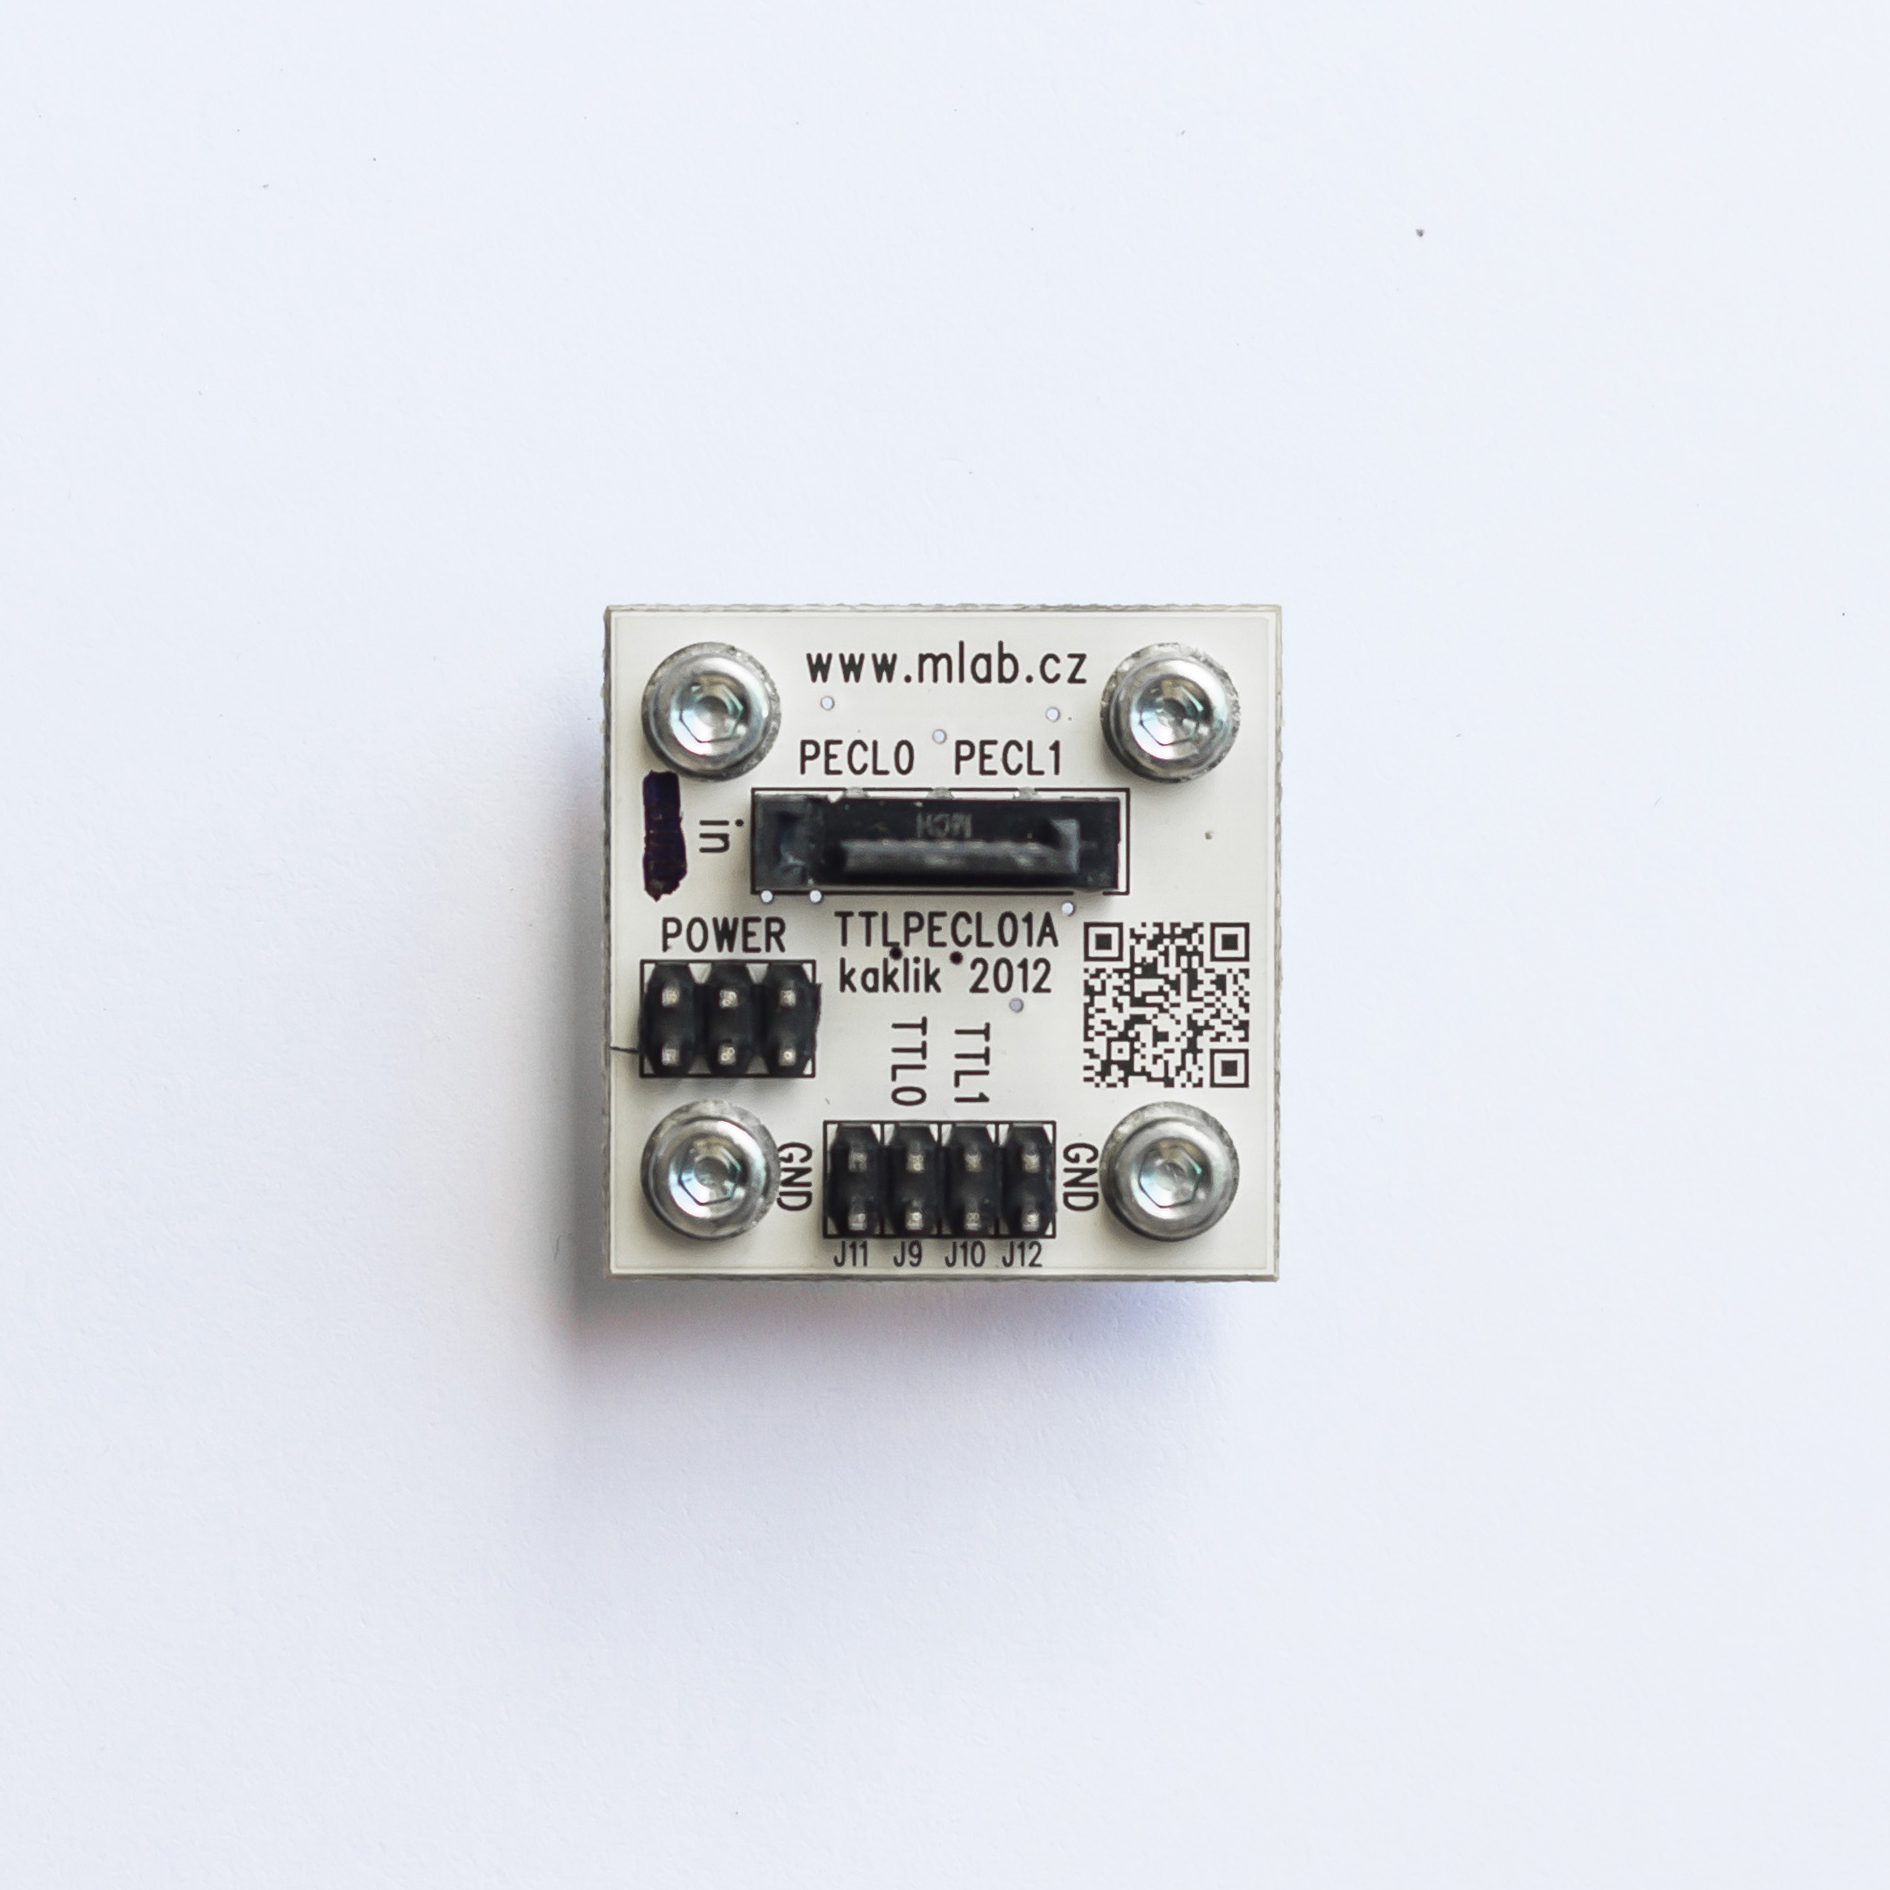
\includegraphics [width=80mm] {./img/TTLPECL01A_Top_Big2.jpg} 
\end{center}
\end{figure}

\begin{figure} [b]

\includegraphics [width=25mm] {./img/TTLPECL01A_QRcode.png} 
\end{figure}

\newpage
\tableofcontents


\section{Technické parametry}
\begin{table}[htbp]
\begin{center}
\begin{tabular}{|c|c|c|}
\hline
\multicolumn{1}{|c|}{Parametr} & \multicolumn{1}{|c|}{Hodnota} & \multicolumn{1}{|c|}{Poznámka} \\ \hline
Napájecí napětí & 3,3 V &  10 mA \\ \hline
Frekvenční rozsah  & 0 - 160 MHz & Pro napájecí napětí 3,3 V \\ \hline
Délka náběžné hrany TTL  & 1 ns & \\ \hline
Délka náběžné hrany PECL  & 500 ps & \\ \hline
\end{tabular}
\end{center}
\end{table}

\newpage
\section{Popis konstrukce}

\begin{itemize}
\item
  Převod TTL na PECL - Realizuje se obvodem
  \href{http://www.micrel.com/page.do?page=/product-info/products/sy10-100elt22l.shtml}{SY100ELT22L}.
\item
  Převod LVPECL na LVTTL - Realizuje se obvodem
  \href{http://www.micrel.com/page.do?page=/product-info/products/sy10-100elt23l.shtml}{SY100ELT23L}.
\end{itemize}
Směr převodu je pak označen přeškrtnutím nežádoucího IN nebo OUT v
potisku modulu vedle SATA konektoru permanentním fixem. Při osazení obvodem SY100ELT23L je na modulu škrtnuto OUT a při osazení modulu obvodem SY100ELT22L je škrtnuto IN. 

\subsection{Zapojení}

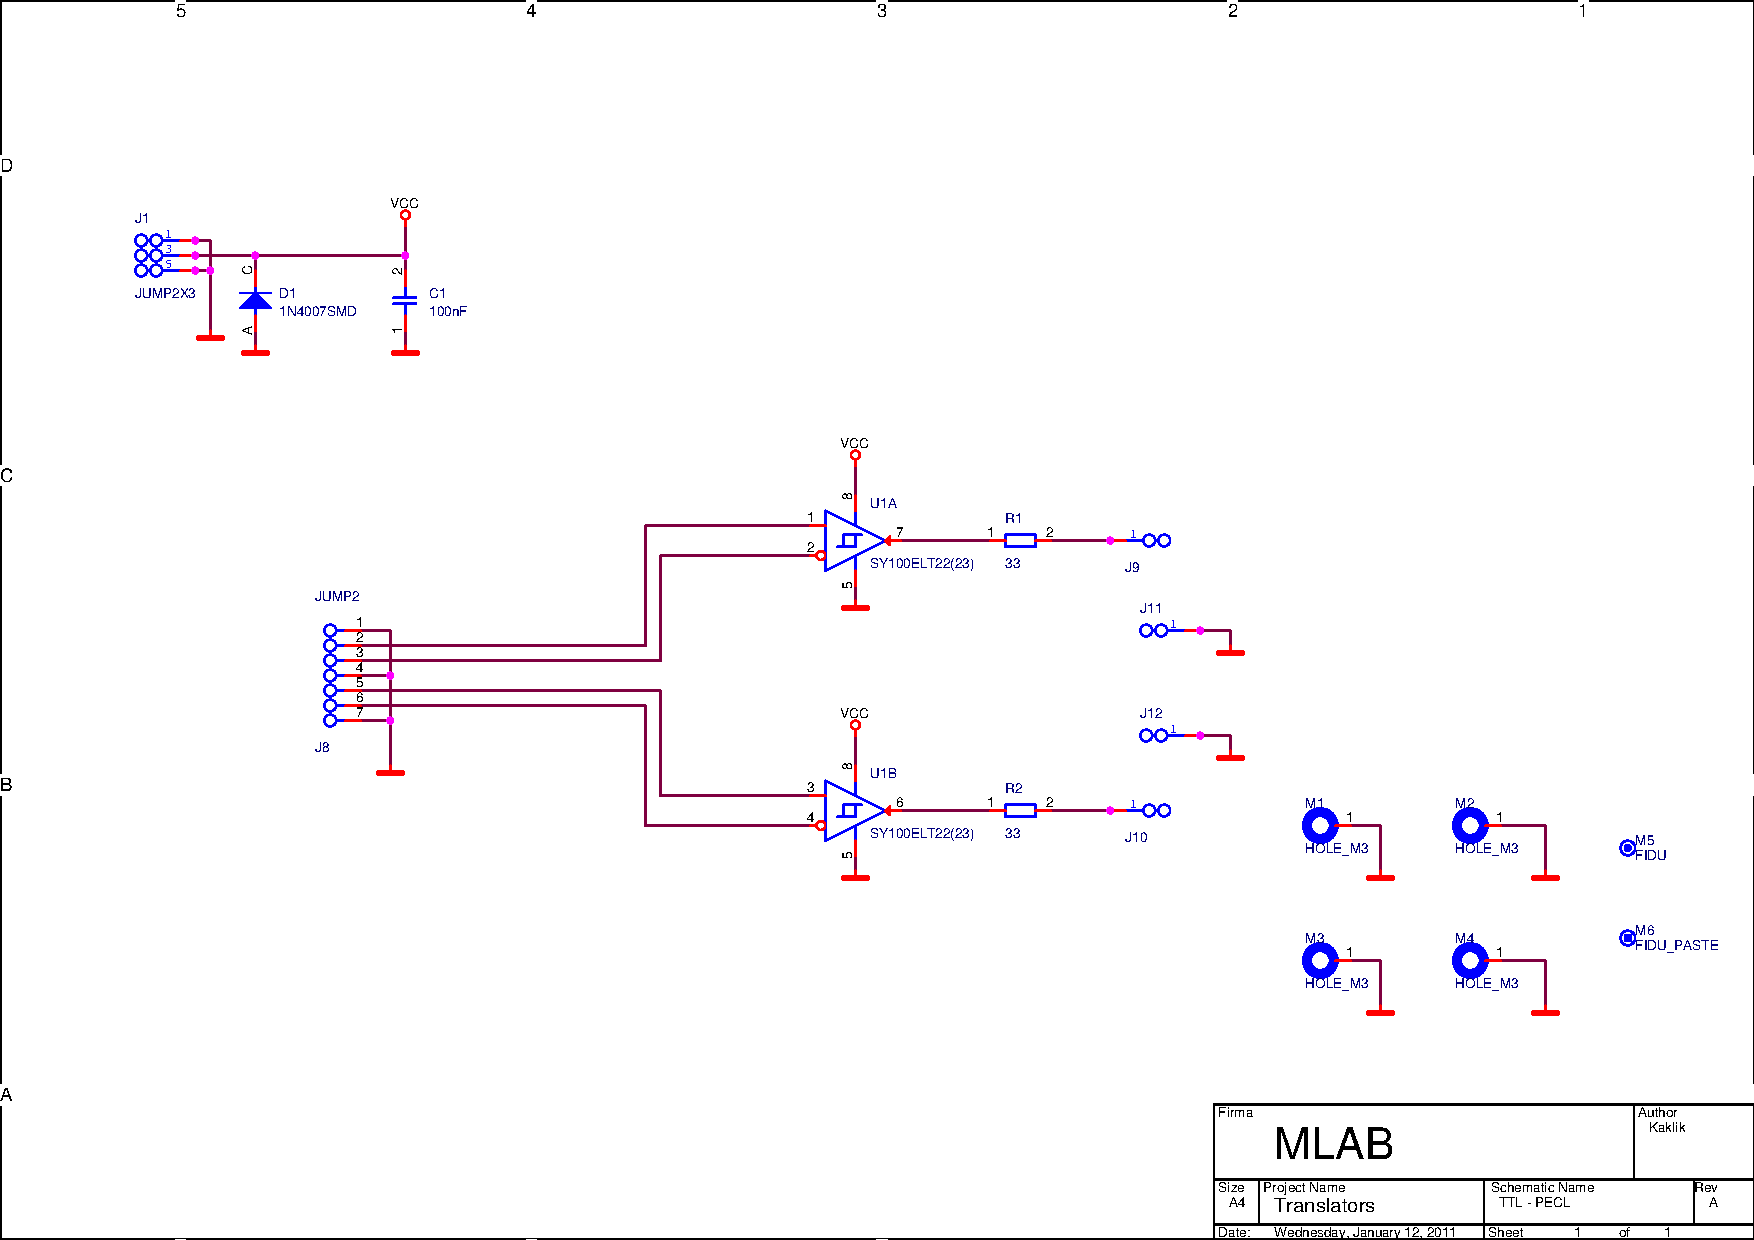
\includepdf[pages={1},landscape=true]{../../SCH/ttlpecl.pdf}

\section{Výroba a testování}

\subsection{Osazení}

\begin{figure} [htbp]
%trim option's parameter order: left bottom right top
  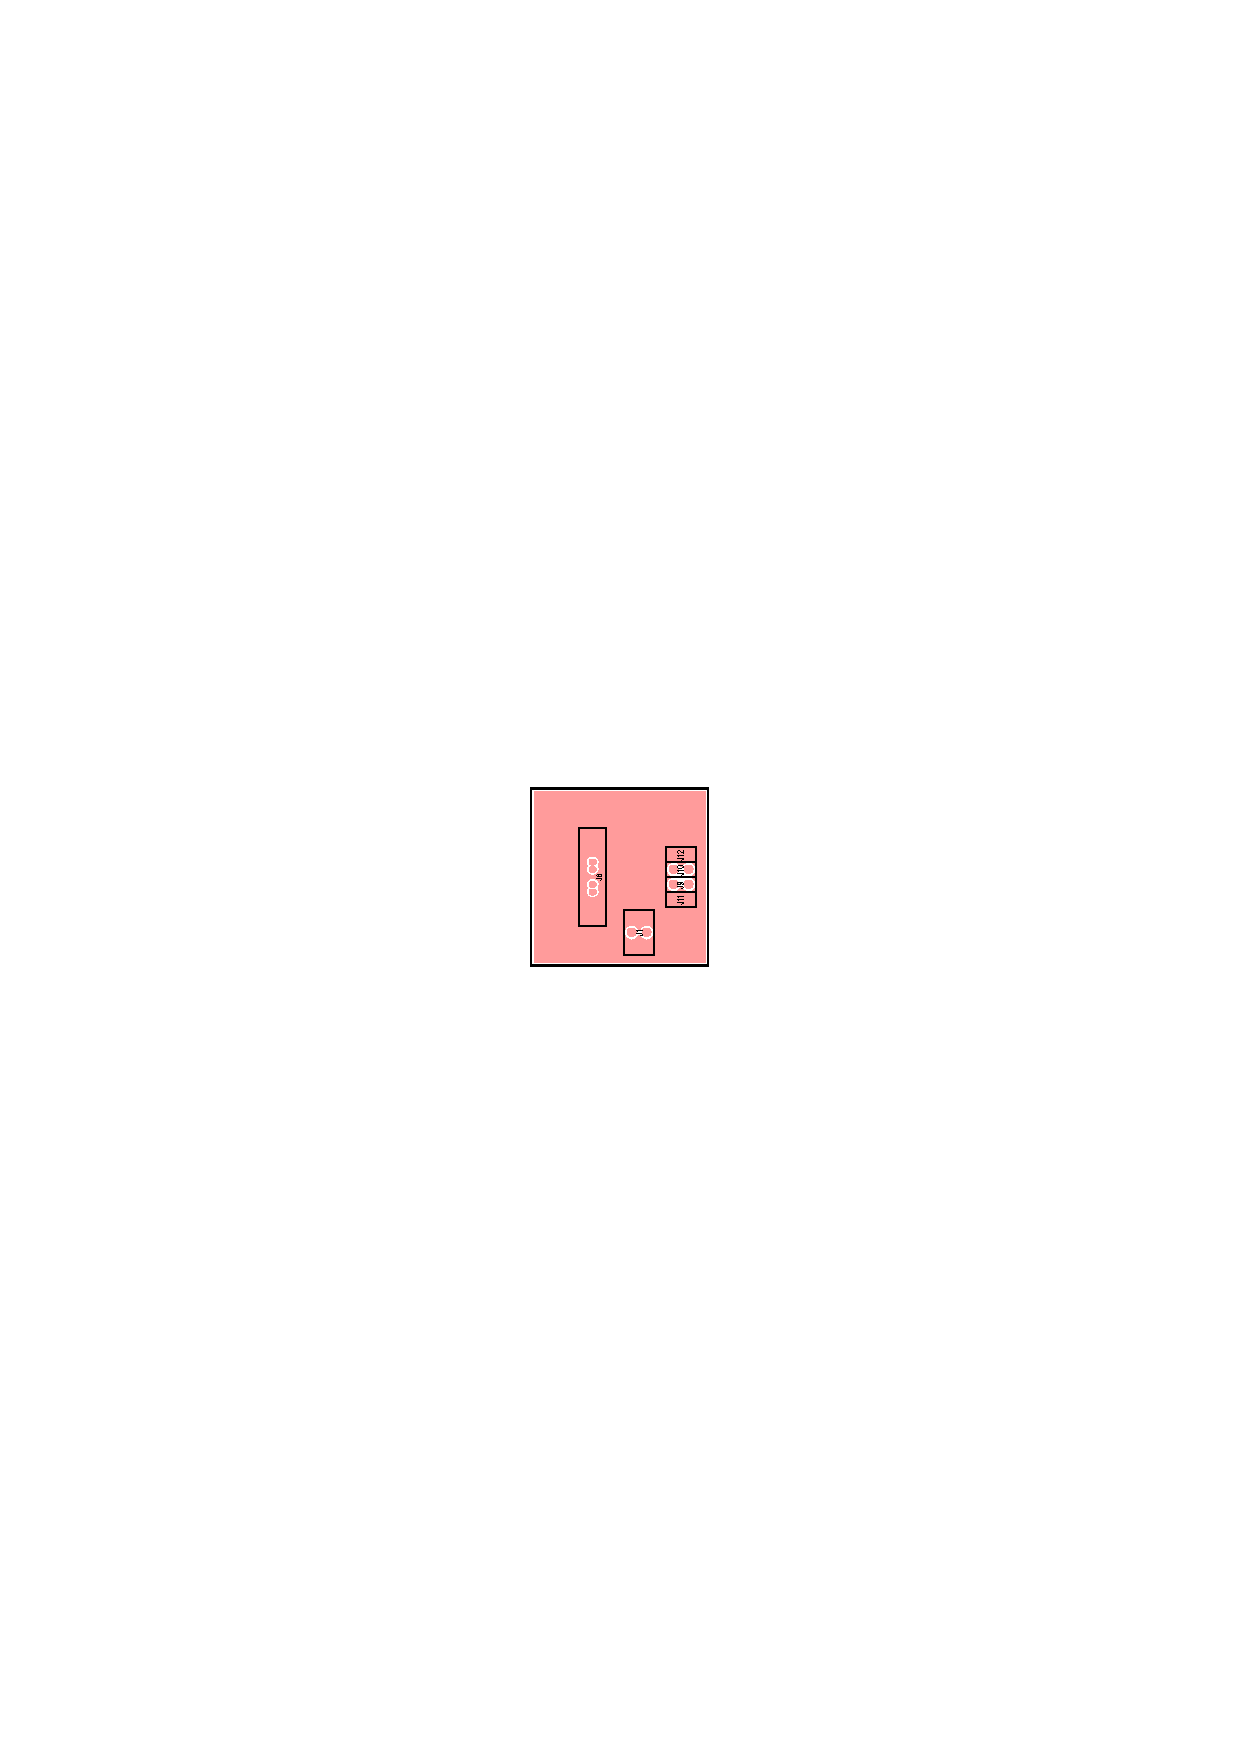
\includegraphics[trim = 85mm 132mm 85mm 132mm, clip, width=8cm]{../../CAM_DOC/O1.pdf}
  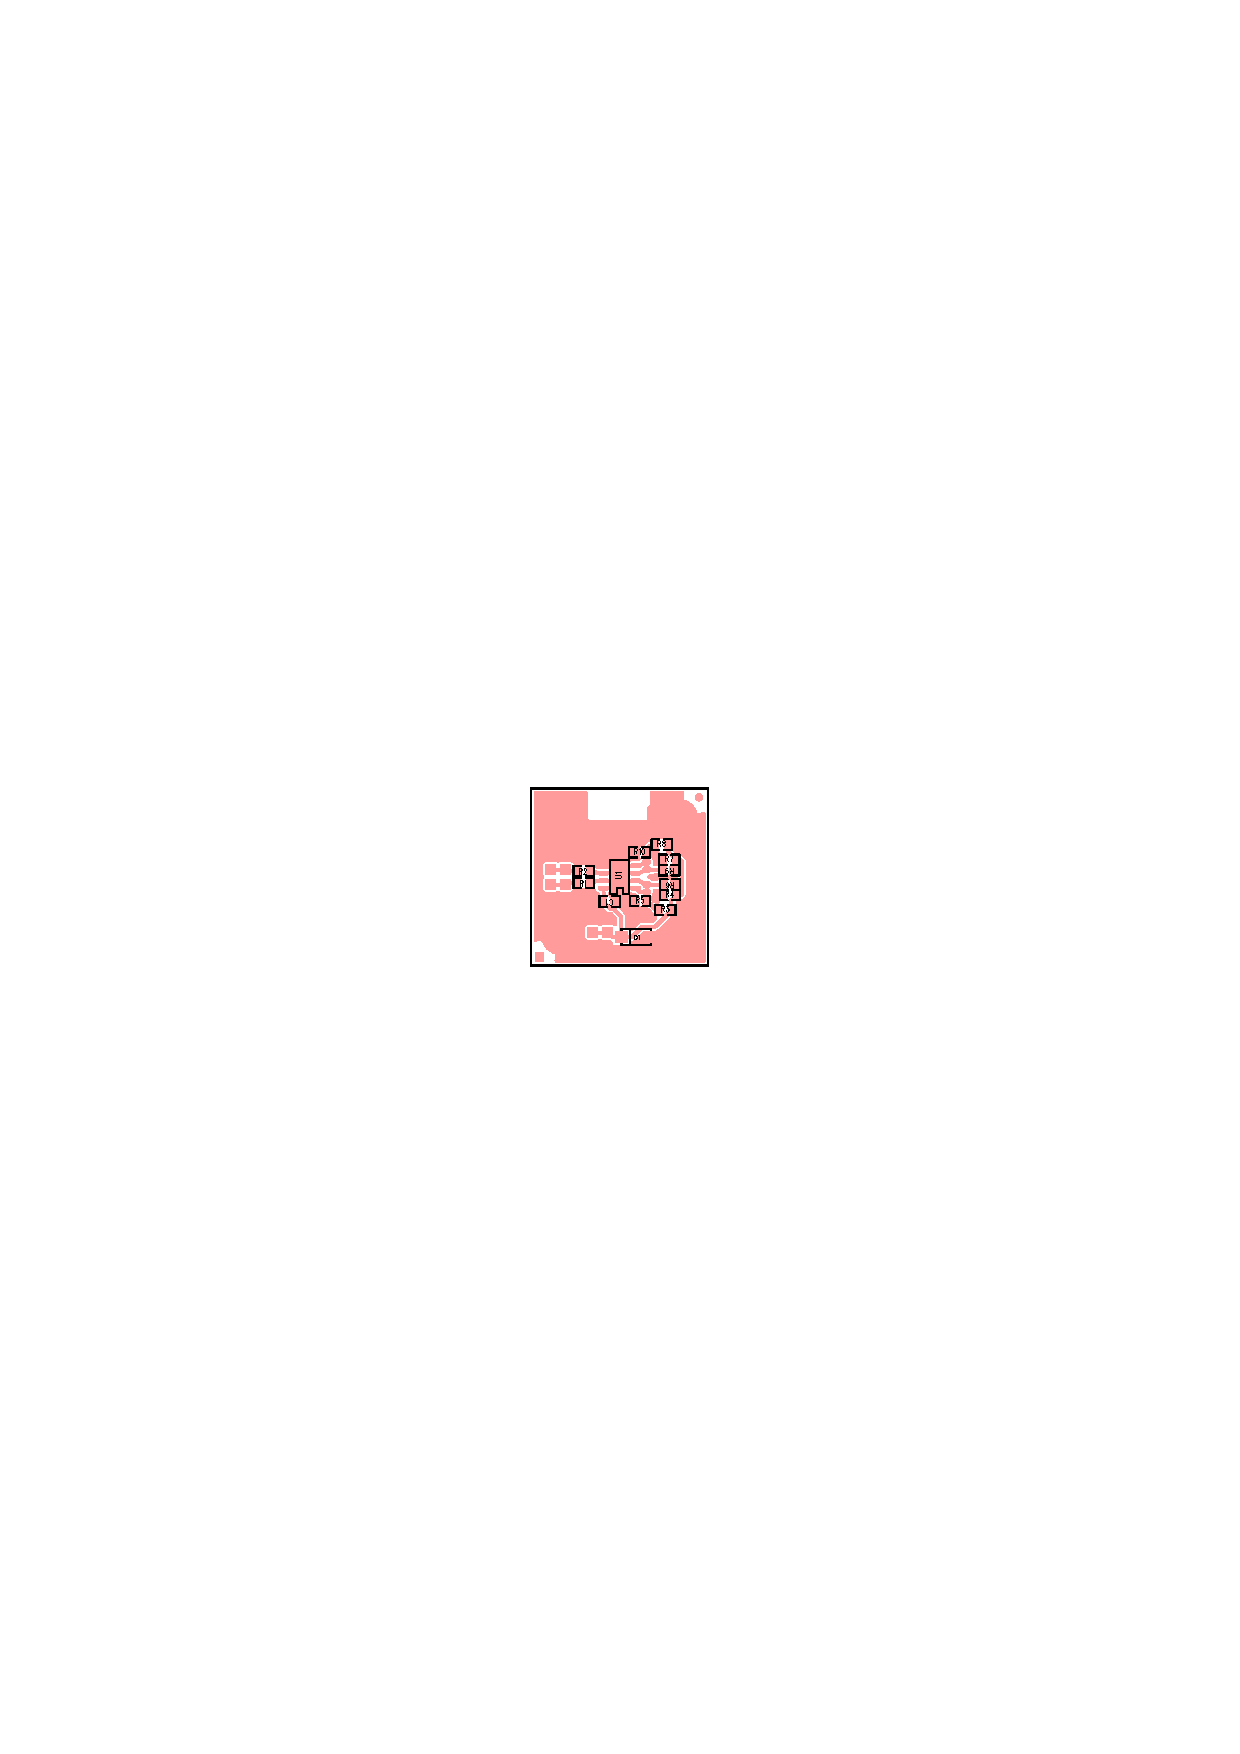
\includegraphics[trim = 85mm 132mm 85mm 132mm, clip, width=8cm]{../../CAM_DOC/O2.pdf}
  \caption{Rozložení součástek na vrchní a spodní straně plošného spoje modulu.}
\end{figure}

\begin{tabular}{ccc}
Označení & Typ & Pouzdro\\ 

\end{tabular} 

\begin{savenotes}
\begin{table}[h!]
\begin{center}
\begin{tabular}{ |c|c|c|c| }
\hline 
Počet & Označení & Typ  & Pouzdro  \\ 
\hline 
1	&	C1	&	100nF	&	SMA \\ 
1	&	D1 	& 	M4 	& 	SMA \\ 
1	&	J1 	& JUMP2X3 &  \\ 
1	& 	J8 	& SATA connector &  \\
1	&	(J9,J10,J11,J12) & JUMP2X4 & \\
2	&	R1,R2	 & 33	& 0805\\
4	& 	R3,R4,R7,R8	&	130 & 0805\\
4	&	R5,R6,R9,R10	&	82 & 0805\\
1	&	U1	&	SY100ELT22(23)\footnote{Konkrétní typ se osazuje podle typu vstupního signálu} & SO8 \\
\hline 
\end{tabular}
\end{center}
\caption{Seznam součástek osazovaných na desku plošného spoje.}
\label{seznam_soucastek_galvanic_isolation}
\end{table}
\end{savenotes}



\subsection{Ověření funkce}

Moduly otestujeme navzájem proti sobě tak, že použijeme variantu modulu pro převod z LVPECL na LVTTL a variantu modulu pro převod LVTTL na LVPECL. Oba moduly pak propojíme SATA kabelem a vyzkoušíme přenos logických úrovní. 


\section{Použití modulu}

\subsection{Napájení}

Napájecí napětí modulu by mělo odpovídat napájecímu napětí související
logiky. A je 3,3V pro LVPECL a LVTTL a +5V pro PECL a TTL logiku. Je ale silně doporučeno moduly používat pouze s napájecím napětím 3,3 V.  

Pozor! V případě použití obvodu SY100ELT23L (Převod LVPECL na LVTTL) je
maximální dovolené napájecí napětí pouze 3,6V! Při jeho překročení může dojít
ke zničení modulu.

\end{document}